\documentclass[a4paper,10pt]{article}
\usepackage{beamerarticle}
\usepackage[T1]{fontenc}
\usepackage[french]{babel}
\usepackage[utf8]{inputenc}
\usepackage{listings}
\usepackage{color}
\usepackage[pdftex,colorlinks=true,urlcolor=blue]{hyperref}
\usepackage{graphics}
\usepackage{graphicx}
\usepackage{ifthen}
\usepackage{fullpage}
\usepackage{times}
\usepackage{fancybox}
\usepackage[english]{qcm}

\renewcommand{\normalfont}{\sffamily} % Pour avoir de "l'arial"
\answerstitle{}

\begin{document}

\begin{center}
  \begin{Large}
    Grundlagen den Programmierung\\
    Revision Quizz\\
  \end{Large}
\end{center}

%\ifbook{

}

\ifslide {

  \begin{frame}{About me...}
    \begin{columns}

    \begin{column}[l]{.3\textwidth}
      \begin{center}
        
\includegraphics[height=120px]{../img/rpe.jpg}
      \end{center}
    \end{column}

    \begin{column}[r]{.7\textwidth}
      \begin{block}{Romain PELISSE}
        \begin{itemize}
          \item \textbf{Middleware Consultant} at \mylink{http://redhat.com}{Red Hat} (2011)
          \begin{itemize}
            \item Architecte Middleware JBOSS
            \item Red Hat Linux Technician
          \end{itemize}
          \item Committer \mylink{http://pmd.sourceforge.net/}{PMD} and \mylink{http://xradar.sourceforge.net/}{XRadar}
          \item Translation for \mylink{http://www.selenic.com/mercurial/wiki/index.cgi/TranslatingMercurial}{HgBook}
          \item Teach build technologies and OPP at \mylink{http://www.esme.fr/}{ESME Sudria}
        \end{itemize}
      \end{block}
    \end{column}
   \end{columns}
 \end{frame}

 \section{Foreword}

 \begin{frame}
   \begin{block}{Some pratical details}
     \begin{itemize}
       \item I have previous experience in teaching, but to \textbf{technical} people or student
       \begin{itemize}
         \item ... so \textit{stop} me, if I go too fast !
       \end{itemize}
       \item I'm French, but I teach in \textbf{English} because my \textit{Deutsch ist schrecklich}
       \item Session last 3 hours, and are divided into:
       \begin{itemize}
         \item 15 minuten: small MCQ (Multiple choice questionnaire), starting next week
         \item ~1 hour
         \item 30" break
         \item ~1 hour
         \item 15" buffer if we are late or need to go deeper
       \end{itemize}
       \item we are here to \textbf{interact}, not to get your ears used to crappy english spoken by
       French people...
     \end{itemize}
   \end{block}
  \end{frame}

  \begin{frame}
    \begin{block}{Sessions agenda}
       \begin{itemize}
         \item 14h00 bis 17h30 - Freitag 04.05 (1/7 - 3h)
         \item 14h00 bis 17h30 - Freitag 11.05 (2/7 - 3h)
         \item 14h00 bis 17h30 - Freitag 25.05 (3/7 - 3h)
         \item 14h00 bis 17h30 - Freitag 01.06 (4/7 - 3h)
         \item \textbf{14h00 bis 17h30 - Freitag 22.06 (5/7 - 3h)}
         \item 14h00 bis 17h30 - Freitag 29.06 (6/7 - 3h)
         \item 14h00 bis 17h30 - Freitag 13.07 (7/7 - 3h)
      \end{itemize}
    \end{block}

    \begin{block}{Be careful !}
      Those dates can changes (and some will probably) - always checkout on Moodle if a session has
      not been rescheduled
    \end{block}
  \end{frame}

  \begin{frame}
    \begin{block}{Goals}
      \begin{itemize}
        \item Basic understanding of how and why program
        \item Impact in \textbf{your} job
        \item Enhance your communication skills with technical people
      \end{itemize}
    \end{block}

    \begin{block}{Who are you ?}
      \begin{itemize}
        \item Quickly gives us an hint of you are and where you come from...
      \end{itemize}
    \end{block}
  \end{frame}

  % classe outline
  \section{How computer works ?}

  \begin{frame}
    \begin{center}
        What do you know about \textbf{how} a computer work ?
    \end{center}
  \end{frame}

  \begin{frame}
   \begin{center}
     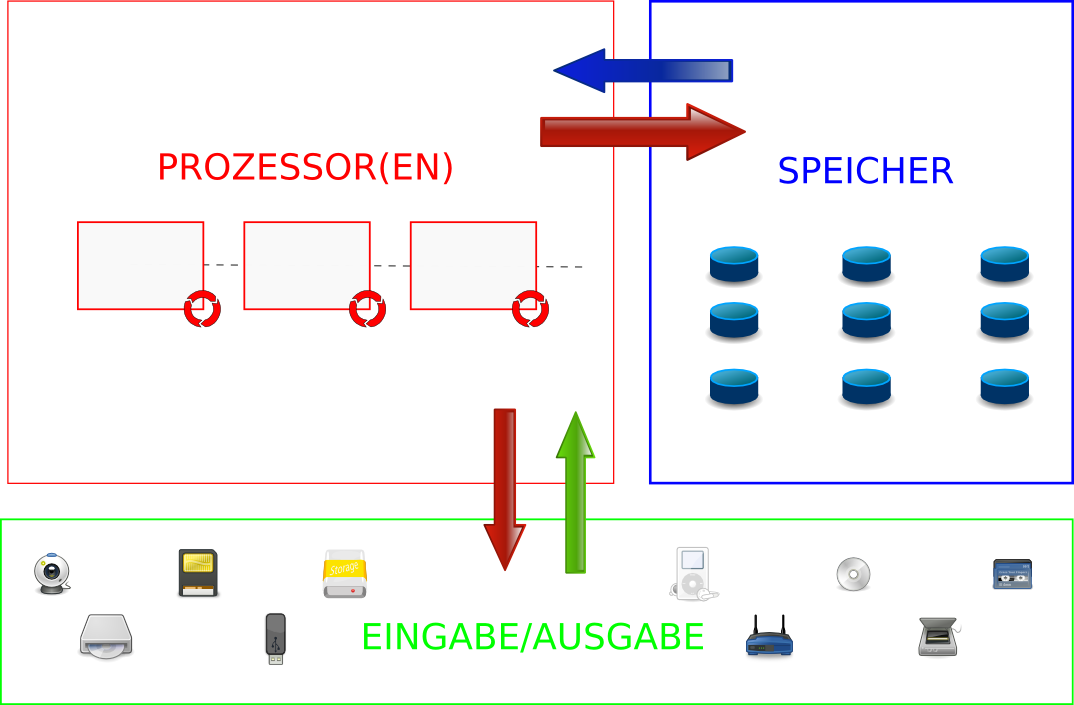
\includegraphics[scale=0.3]{img/cpu-schematics.png}
   \end{center}
  \end{frame}

  \begin{frame}
    \begin{center}
      \begin{itemize}
        \item What is an \textbf{operating system}(OS) ?
        \item Name a few OS names that you know of ?
        \item What does exactly an operating system ? What are its \textbf{responsabilities}?
      \end{itemize}
    \end{center}
  \end{frame}

  \begin{frame}{Role of an Operating System}
    \begin{center}
      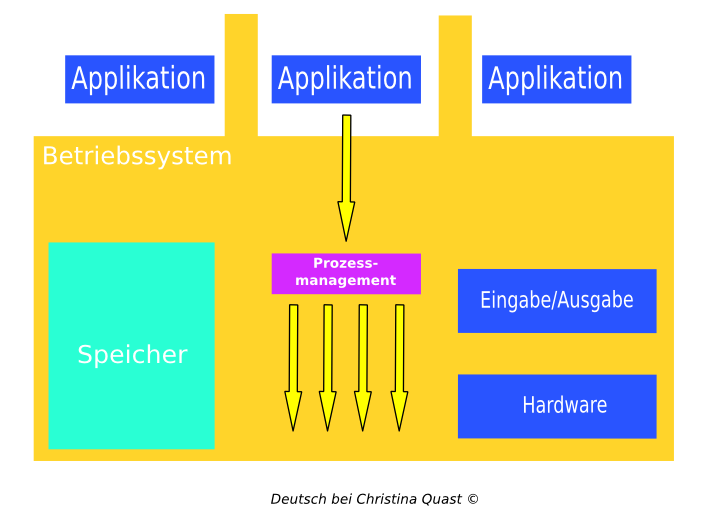
\includegraphics[scale=0.3]{img/operating-system.png}
    \end{center}
  \end{frame}

  \begin{frame}{Speed of I/Os}
    \begin{center}
      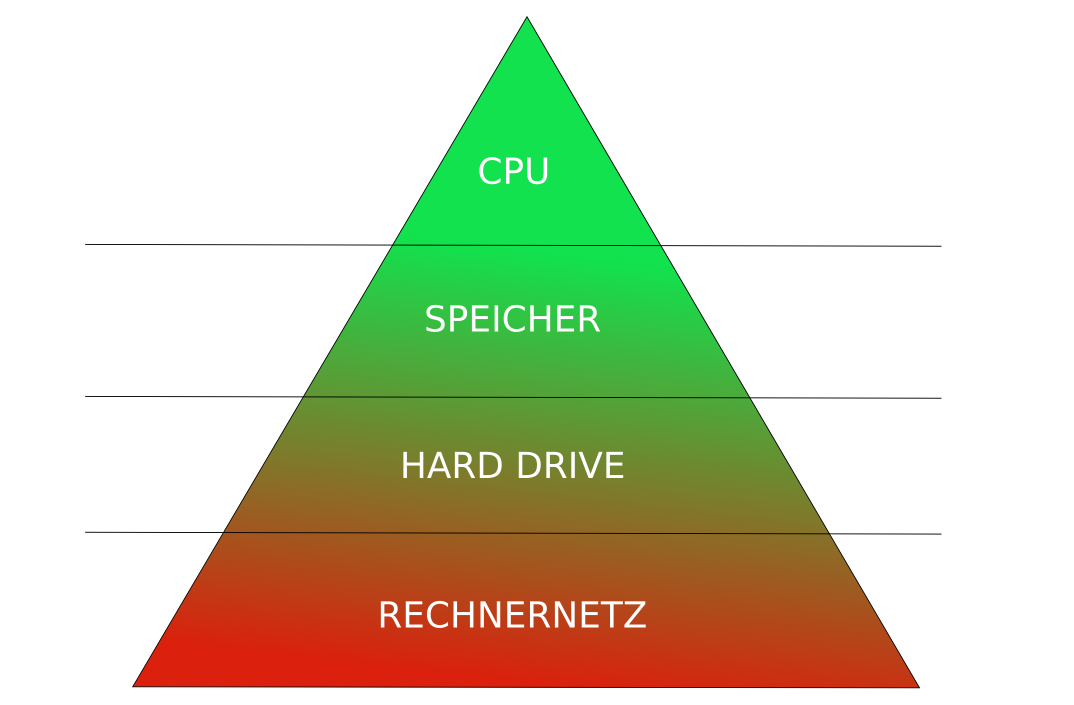
\includegraphics[scale=0.3]{img/pyramid-io.png}
    \end{center}
  \end{frame}

  \section{Short history of IT}

  \begin{frame}{First era of IT: Mainframe and terminals}
    \begin{center}
      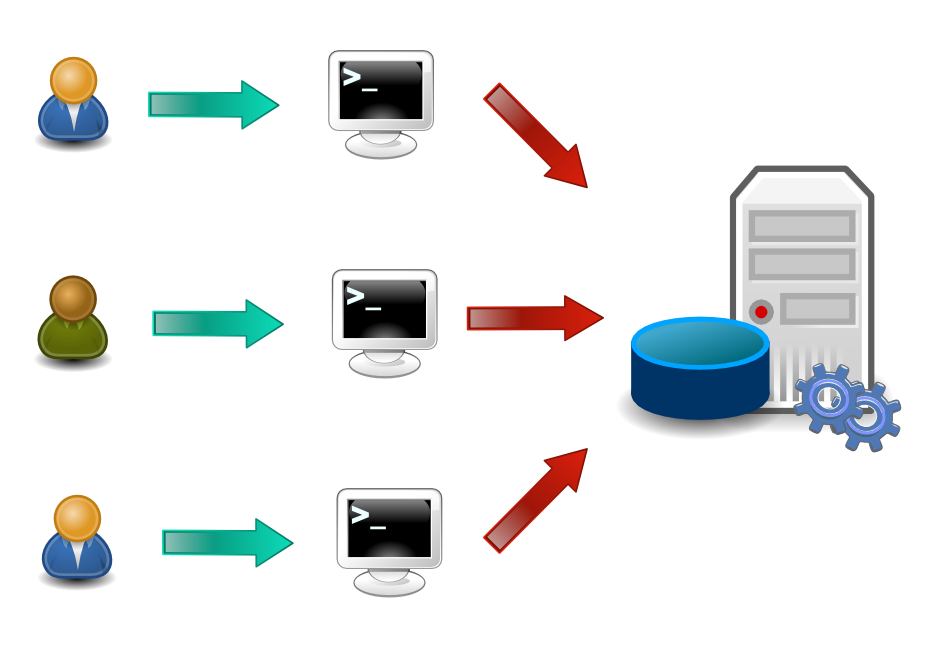
\includegraphics[scale=0.3]{img/mainframe-terminals.png}
    \end{center}
  \end{frame}

  \begin{frame}{Second era of IT: Clients and servers}
    \begin{center}
      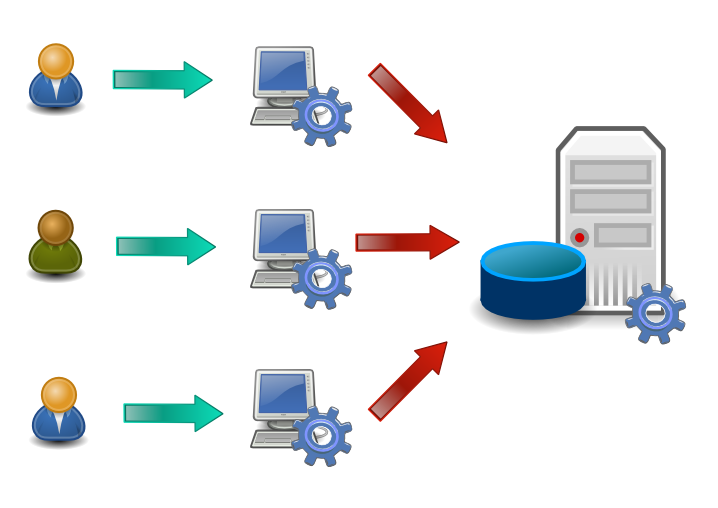
\includegraphics[scale=0.3]{img/fat-clients.png}
    \end{center}
  \end{frame}

  \begin{frame}{Third era of IT: The Internet}
    \begin{center}
      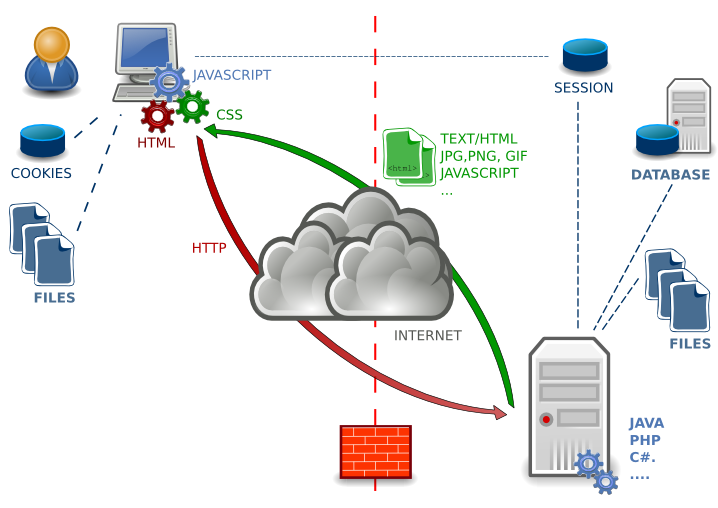
\includegraphics[scale=0.3]{img/internet.png}
    \end{center}
  \end{frame}

  \begin{frame}{Data persistance}
    \begin{center}
      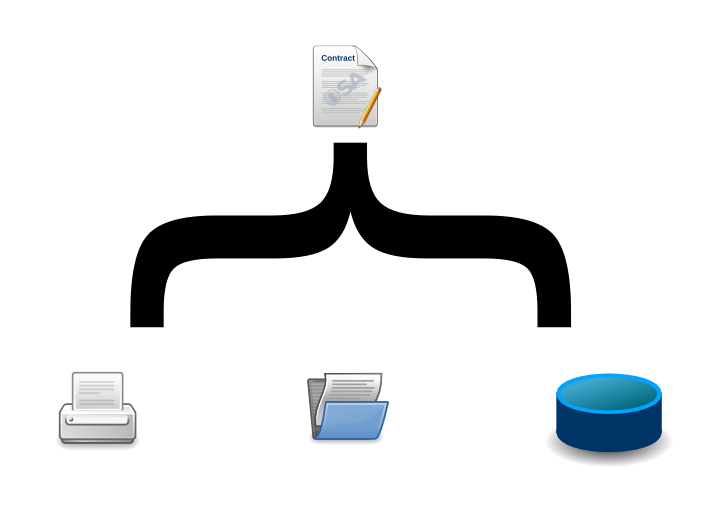
\includegraphics[scale=0.3]{img/persistance.png}
    \end{center}
  \end{frame}

  \section{Java}

  \begin{frame}{Java}
    \begin{block}{What is Java ?}
      \begin{itemize}
        \item \textbf{programming} language
        \begin{itemize}
          \item "look-like" C code
          \item \textbf{Object Programming Oriented}
          \item strongly \textbf{structured}
        \end{itemize}
        \item operating system \textbf{independant}
        \item running within a \textbf{virtual machine}
        \item with automated memory collection
      \end{itemize}
    \end{block}

    \begin{center}
      
\includegraphics[scale=0.2]{img/java-logo.jpg}
    \end{center}
  \end{frame}

  \begin{frame}{Java}
    \begin{block}{Compiling code....}
      \begin{itemize}
        \item What for ? What does it do ? What does it bring ?
        \item Must all languages be compiled ?
        \item If not, what is the point of compiled language ?
      \end{itemize}
    \end{block}
  \end{frame}

  \begin{frame}{Java}
    \begin{block}{The infamous Hello The World program...}
      \begin{itemize}
        \item What is this program ? What does it do ?
        \item Why does programmer always start by writing such a program ?
        \item Let's see how to implement such a program in Java...
      \end{itemize}
    \end{block}
  \end{frame}
}

%\ifbook{

}

\ifslide{
 \section{Brief reminder - multiple choice}

 % TODO

  \section{Agenda}
  \begin{frame}{Agenda}
    \begin{block}{Session outline}
      \begin{itemize}
        \item Hello World
        \item Java syntax and purpose of a syntax
        \item Identifier
        \item Comments
        \item Core data types
        \item Operators
        \item Strings
      \end{itemize}
    \end{block}
  \end{frame}

  \section{The Hello World}

  \begin{frame}{First program in Java}
    \begin{block}{Instructions}
      \begin{itemize}
        \item Download the HelloWorld.java file and save it on the Desktop
        \item Start a \textbf{Terminal} in the application menu
        \item Change the current directory of the terminal by using the following command:
        \begin{itemize}
          \item \texttt{pwd} - prints current directory
          \item \texttt{ls} - displays the files of the directory
          \item \texttt{cd <directory>} - change to directory provided as arguments
          \item \texttt{man <command>} - help for the command
        \end{itemize}
        \item Once the current directory of the Terminal is Desktop, compile the file:
        \begin{itemize}
          \item \texttt{\$ javac HelloWorld.java}
        \end{itemize}
        \item Once the code has compiled, execute it:
        \begin{itemize}
          \item \texttt{\$ java HelloWorld}
        \end{itemize}
      \end{itemize}
    \end{block}
  \end{frame}

  \begin{frame}{Results}
   \begin{center}
     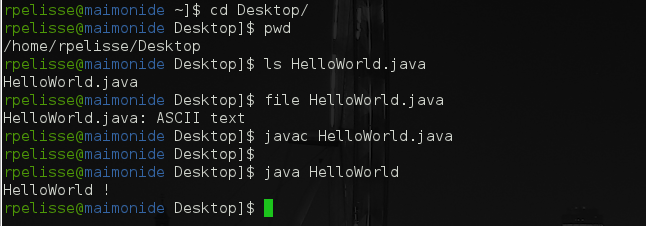
\includegraphics[scale=0.5]{img/hello-world.png}
   \end{center}
  \end{frame}

  \begin{frame}{Communicating with the program}
    \begin{block}{Arguments}
      \begin{itemize}
        \item Download the Arguments.java file and save it on the Desktop
        \item Compile and execute the program, adding some arguments:
        \item \texttt{\$ java Argument The answer is 42.}
      \end{itemize}
    \end{block}
    \begin{center}
      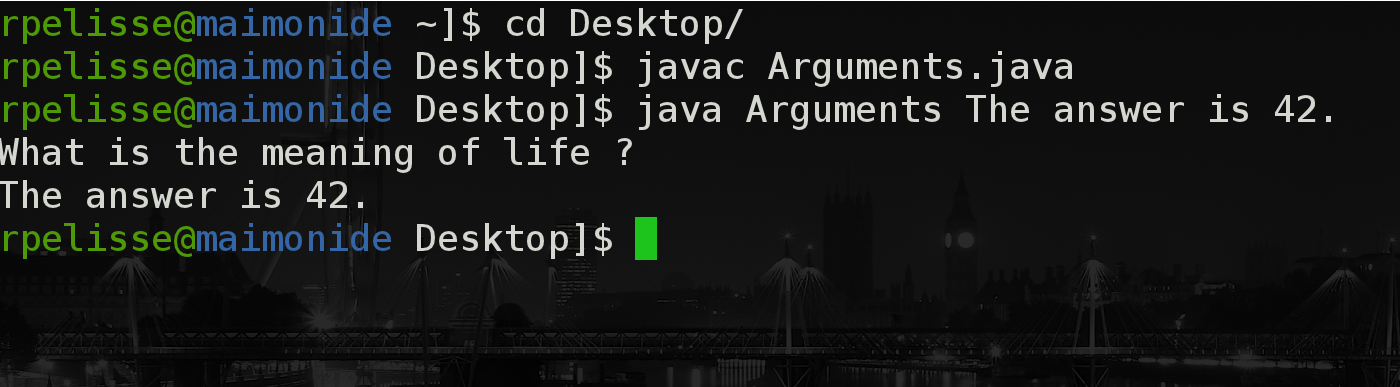
\includegraphics[scale=0.2]{img/arguments.png}
    \end{center}
  \end{frame}

  \section{Java and its syntax}
  \subsection{File organization}
  \begin{frame}
    \begin{block}{What does a source file contains ?}
      \begin{itemize}
        \item look at the HelloWorld class and identify the different section:
        \begin{itemize}
          \item header
          \item comment
          \item class name
        \end{itemize}
      \end{itemize}
    \end{block}
    \begin{center}
      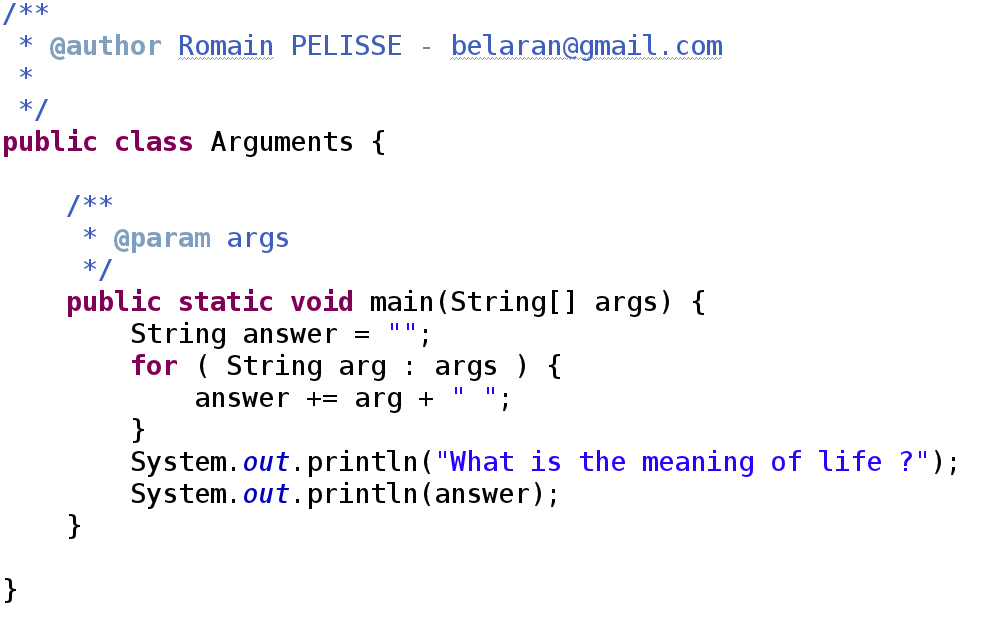
\includegraphics[scale=0.2]{img/java-source-file.png}
    \end{center}
  \end{frame}
  \subsection{Variables}
  \begin{frame}
    \begin{block}{Variable - how to store and manipulate data}
      \begin{itemize}
        \item What is a variable ?
        \begin{itemize}
          \item memory allocation to store date
          \item the data is \textbf{typed}
        \end{itemize}
        \item What can do with them ?
        \begin{itemize}
          \item change the value
          \item use operator
        \end{itemize}
      \end{itemize}
    \end{block}
    \begin{center}
      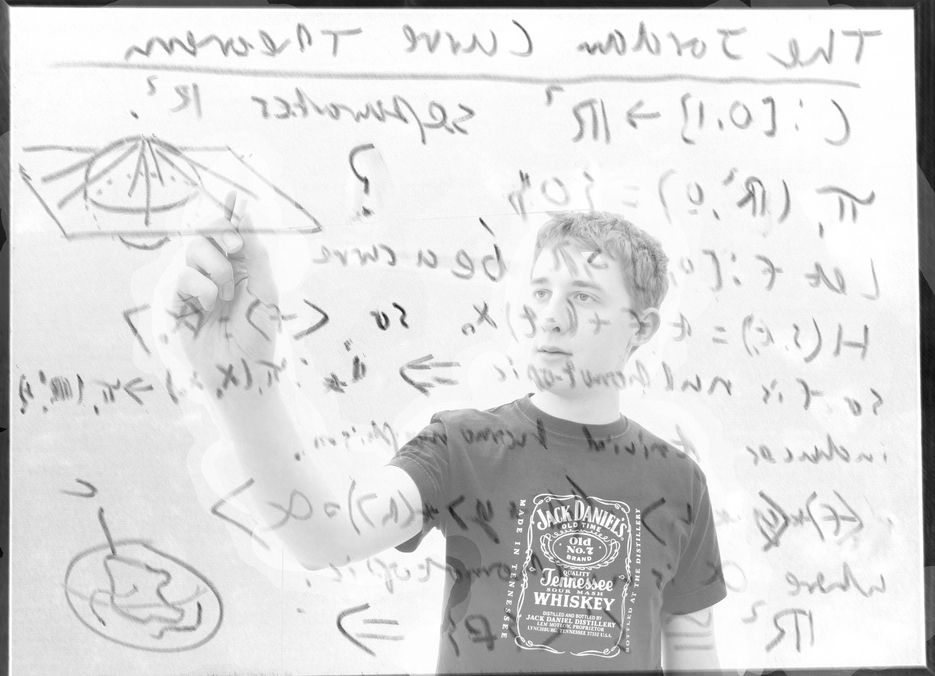
\includegraphics[scale=0.2]{img/variables.jpg}
    \end{center}
  \end{frame}

  \begin{frame}
    \begin{block}{Java primitives}
      % what the point of short, double if we generally use int ?
      % what are the "risk" or advantages of using short or long ?
      % why use boolean over an int with 0,1 ?
      \begin{description}
        \item[byte] an 8-bit signed integer - value range: -128 to 127 (inclusive)
        \item[short] a 16-bit signed  integer - value range:-32,768 to 32,767 (inclusive)
        \item[int] a 32-bit signed - value range: -2,147,483,648 to 2,147,483,647 (inclusive)
        \item[long] a 64-bit signed - value range: -9,223,372,036,854,775,808 to 9,223,372,036,854,775,807 (inclusive)
        \item[float] a single-precision 32-bit IEEE 754 floating point.
        \item[double] a double-precision 64-bit IEEE 754 floating point
        \item[boolean] has only two possible values: true and false
        \item[char] a single 16-bit Unicode character
      \end{description}
    \end{block}
  \end{frame}
  \subsection{Operator}
  \begin{frame}
    \begin{block}{Playing with variables - Operator}
      \begin{itemize}
        \item Download the Addition.java file and save it on the Desktop
        \item Compile it and execute it:
        \begin{itemize}
          \item \texttt{\$ java Addition 1 2}
        \end{itemize}
        \item Exercices:
        \begin{itemize}
          \item copy this file and rename it \textbf{Substract.java} - change this new file to
          implement a substraction
          \item in \textbf{Addition.java}, replace the \texttt{int} by \texttt{short} and run the
          program with inputs 5 and 128. What is happening ? Why ?
          \item do we really need \textbf{variables} for this program ? How can we do
          \textbf{without} using variables ?
          \item adapt \textbf{Addition.java} in order to have the program able to do addition with
          \textbf{money}
        \end{itemize}
      \end{itemize}
    \end{block}
  \end{frame}

  % Introducing the "useless" data type => character

  % Function calls

}

\ifslide{

  \section{Agenda}
  \begin{frame}{Agenda}
    \begin{block}{Session outline}
      \begin{itemize}
        \item how to use an IDE (Eclipse)
        \item control structure (if, for, while, .switch,...)
        \item functions
        \item error handling
      \end{itemize}
    \end{block}
  \end{frame}

  \section{Using an IDE: Eclipse}

  \begin{frame}{What is an Integrated Development Environment ?}
    \begin{block}{Main features}
      \begin{itemize}
        \item Advanced file editing
        \begin{itemize}
          \item highlight syntax with colors
          \item syntax checker
          \item auto completion
        \end{itemize}
        \item Program building
        \begin{itemize}
          \item compilation
          \item run program inside the IDE
        \end{itemize}
        \item \textbf{debugger}
        \begin{itemize}
          \item execute program \textbf{interactively}
          \item expose variables content, allow to modify them direclty
        \end{itemize}
      \end{itemize}
    \end{block}
  \end{frame}
}

\ifslide{
  \begin{frame}{A short Eclipse Tutorial}
    \begin{block}{Eclipse IDE}
      \begin{itemize}
        \item Open Source, java based, IDE
        \item Most used IDE in the World
        \item Focus on Java programming but also used for other technologies
        \item Cross platform program
        \item Speed up development (up to 40\% !)
      \end{itemize}
    \end{block}
  \end{frame}


  \begin{frame}{Use Eclipse (1/2)}
    \begin{block}{Instructions}
      \begin{itemize}
        \item Look for Eclipse in the Application launcher menu, and start it
        \item Eclipse will ask for the location of the \textbf{workspace}
        \begin{itemize}
          \item this location is where Eclipse stores the project's files
          \item simply click on "OK" and accept the default location
        \end{itemize}
        \item Go to File->New->Java Project to create a new, empty, Java project.
        \item Use your first and lastname (ex:romain-pelisse) as project name and click sur "Finish"
        \item \textbf{Right-click} on the folder 'src' and select the 'import' options:
        \begin{itemize}
          \item a wizard will appear to specifify the import method
          \item select General->File System and click on "Next"
          \item use the "Browser" button to select the "Desktop" folder
          \item select all the java sources files (.java) on Deskopt (all files from the previous
          session)
          \item click on "Finish" to import all of them
        \end{itemize}
      \end{itemize}
    \end{block}
  \end{frame}

  \begin{frame}{Use Eclipse (2/2)}
    \begin{block}{Instructions}
      \begin{itemize}
        \item Compile, run and \textbf{debug}:
        \begin{itemize}
          \item Eclipse will compile for you, automatically any Java files in the src/ folder -
          nothing to do !
          \item To run a Java file, right-click on the file and select Run as->Java Application
          \item To Debug a program, right-click on the file and select Debug as->Java Application
        \end{itemize}
      \end{itemize}
    \end{block}
  \end{frame}
}

\ifslide {
  \begin{frame}{Use Eclipse's debugger}
    \begin{block}{Instructions}
      \begin{itemize}
        \item Double click on the column on the left of the source code to set a \textbf{breakpoint} - see picture below
        \item Run the program with the debugger (Debug as->Java Application) and ...
        \begin{itemize}
          \item run the program step-by-step
          \item examine the values of each available variables
          \item set a breakpoint and execute the program up to it
        \end{itemize}
      \end{itemize}
    \end{block}
  \end{frame}

   \section{Control Structure}

   \begin{frame}{The 'if' statement}
     \begin{block}{The 'if' statement}
      \begin{itemize}
        \item simple form of control flow statement.
        \item directs the program to execute a certain section of code...
        \item ...if and only if the test evaluates to true
        \item in Java, a the test must be boolean expression.
       \end{itemize}
     \end{block}

     \begin{block}{Instructions}
       \begin{itemize}
         \item Download the HowToUseIfStmt.java file and save it on the Desktop
         \item Import the file in your project as you did before
         \item Implements the program as defined in the source file
         \item To add an 'if' statement to the code, use the autocompletion feature of Eclipse
         (crtl+space)
       \end{itemize}
     \end{block}
   \end{frame}

}

\ifslide{
   \begin{frame}{The 'for' statement}
     \begin{block}{The 'for' statement}
      \begin{itemize}
        \item execute a block of code continuously
        \item consists of tree parts :\tiny{
        \begin{description}
          \item[initialization]: an expression that sets the value of the loop control variable,
          executed only once.
          \item[condition]:  a boolean expression that tests the loop control variable against a target
          value and hence works as a loop terminator.
          \item[Increment/decrement]: an expression that increments or decrements the loop
          control variable.
        \end{description}
        }
       \end{itemize}
     \end{block}

     \begin{block}{Instructions}
       \begin{itemize}
         \item Using Eclipse, copy the file HowToUseIfStmt.java to HowToUseForLoop.java
         \item This new program accepts only one character values as arguments:\texttt{java
         HowToUseForLoop 1 2 3 4 5 6 7} - there no more bound for the number of arguments.
         \item Modify the program accordingly
         \item To add a 'for' statement to the code, use the autocompletion feature of Eclipse
         (crtl+space)
       \end{itemize}
     \end{block}
   \end{frame}

   \begin{frame}{The 'while' statement}
     \begin{block}{The 'while' statement}
       \begin{itemize}
         \item execute a block of code continuously...
         \item ... as long as the condition is true.
         \item mix between an 'if' and a 'while'
         \item a \mylink{http://www.roseindia.net/java/beginners/DoWhile.shtml}{do...while} statement also exist - to skip the first evaluation.
       \end{itemize}
     \end{block}

     \begin{block}{Instructions}
       \begin{itemize}
         \item Download the file WhyWhileStmtAreAlsoCool.java
         \item Modify the program as requested in the code
       \end{itemize}
     \end{block}
   \end{frame}
}

\ifslide{
   \begin{frame}{The 'switch' statement}
     \begin{block}{The 'switch' statement}
      \begin{itemize}
        \item an alternative to a series of 'else if'
        \item allows for any number of possible execution paths
        \item works with the byte, short, char, and int primitive data types
        \item works with enumerated types (we'll see them later)
        \item body of a switch statement is known as a switch block.
        \item Any statement immediately contained by the switch block may be labeled:
        \begin{itemize}
          \item with one label
          \item several lables
          \item or the default label
        \end{itemize}
      \end{itemize}
     \end{block}

     \begin{block}{Remarks}
       \begin{itemize}
         \item powerful but rather complex
         \item seldom used
         \item generally just to remove a messy, long if statement
       \end{itemize}
     \end{block}
   \end{frame}
}

\section{Functions}

\ifslide{
  \begin{frame}
    \begin{block}{What is function ?}
       \textit{In computer science, a subroutine, also termed procedure, function, routine, method, or
       subprogram, is a part of source code within a larger computer program that performs a specific
       task and is relatively independent of the remaining code. - Wikipedia
       \mylink{http://en.wikipedia.org/wiki/Subroutine}{"Subroutine"}, accessed
       the 22.05.2012}
    \end{block}

    \begin{block}{What are their purpose ?}
      \begin{itemize}
        \item reuse code easily
        \item make code easier to read
        \item breakdown code in different, meaningful, part
        \item hide complexity
      \end{itemize}
    \end{block}
  \end{frame}

  \begin{frame}
    \begin{block}{Functions syntax}
      \begin{center}
        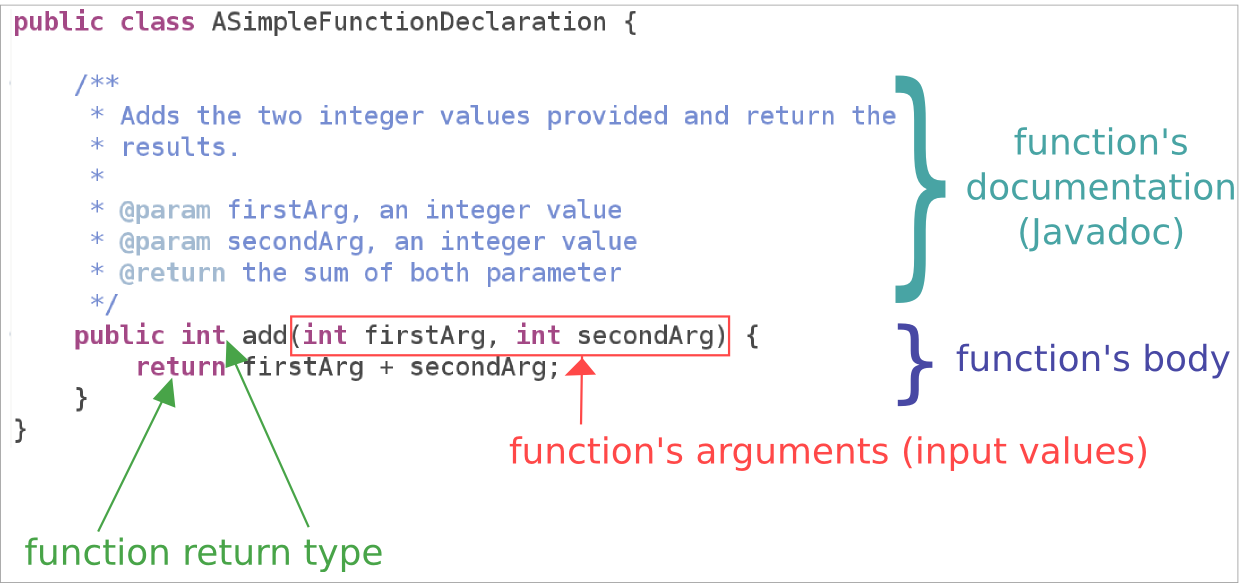
\includegraphics[scale=0.2]{../img/a-simple-java-function.png}
      \end{center}
    \end{block}

    \begin{block}{Instructions}
      \begin{itemize}
        \item Download and import the file called LenghtyProgram
        \item Modify the code according to the instruction
      \end{itemize}
    \end{block}
  \end{frame}
}

\section{Error Handling}
\ifslide{
 \begin{frame}
    \begin{block}{Structure to handle error in programming language}
      \begin{itemize}
        \item do nothing
        \begin{itemize}
          \item program crashes
          \item no information on the root cause
        \end{itemize}
        \item use "status code"
        \begin{itemize}
          \item functions can't return value
          \item leads to message such as "Error 400 happened"
          \item needs to have an error database to translate the status code
        \end{itemize}
        \item return a complete structure describing in length the error
        \begin{itemize}
          \item ideal, but...
          \item ...still remove the option of having returning value
        \end{itemize}
      \end{itemize}
    \end{block}
 \end{frame}
}


\end{document}
